\documentclass[11pt,titlepage]{article}
\usepackage{graphicx}
\def \rms {{\it rms}\ }
\def\parhead#1#2#3{#1\>#2\>\`#3\\}
\def\parlist#1{\smallskip \hspace{10mm} \begin{minipage}{150mm}#1\end{minipage}\\}
\def\pararg#1#2{\>#1\>\begin{minipage}[t]{83mm}#2\end{minipage}\\}
\parskip=2mm
\parindent=0mm
\textheight=240mm
\textwidth=160mm
\oddsidemargin=0mm
\evensidemargin=8mm
\topmargin=-10mm
\itemsep=-1mm
\topsep=0mm
\begin{document}
\title{
\vspace{-3cm}
{\Huge EyE
%\psfig{figure=draft.ps,width=8cm,rwidth=0cm,rheight=0cm}
}\\
{\huge $v1.1$}\\\vspace{1cm}
{\LARGE User's guide}\vspace{1cm}}
\date{\today\\\vspace{1cm}\centerline{\fbox{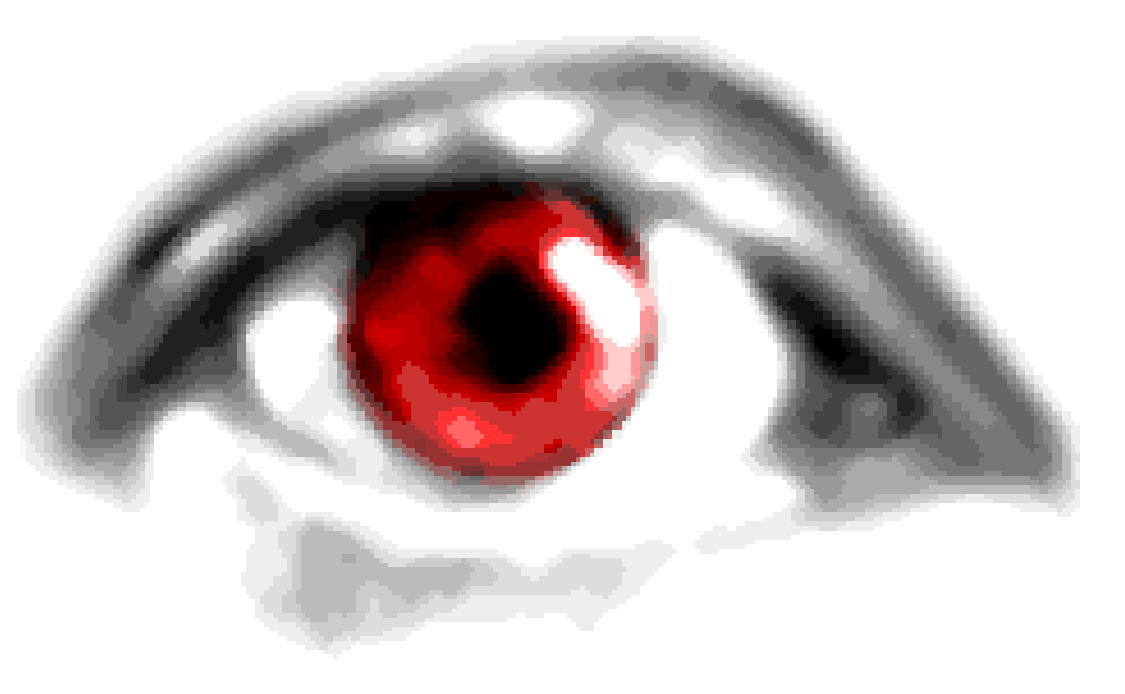
\includegraphics[width=15cm]{ps/eyeintro.ps}}}}
\author{{\Large E. BERTIN}\\Institut d'Astrophysique \& Observatoire de Paris\\{\ }\\
{\Large C.MARMO}\\Institut d'Astrophysique de Paris}
\maketitle
\newpage
\pagestyle{empty}
\setcounter{page}{0}
{\ }
\newpage
\pagestyle{plain}
\pagenumbering{roman}
\tableofcontents
\newpage
{\ }
\newpage
\pagenumbering{arabic}
\section{What is {\sc EyE}?}
{\sc EyE} ({\em Enhance Your Extraction}) is a program that generates non-linear image filters using machine-learning.
A neural network, connected to pixels of a moving window (``retina'') in one or several input image(s), is trained to associate
these ``stimuli'' to the corresponding response in one or several ``model'' image(s). The resulting filter can then be loaded in
SExtractor (Bertin 1999) to operate complex, wildly non-linear filters on astronomical images. Typical applications of
this system include adaptive filtering, feature detection and cosmetic corrections. The main features of the {\sc EyE} are:
\begin{itemize}
\item FITS format, including Multiple Extensions, is used for input and output,
\item Ability to work with very large images (up to, say, $10^8 \times 10^9$ pixels on a 64 bits workstation),
\item Automatic selection of representative pattern pairs,
\item Adaptive compression/expansion of the input/output signals to comply with the lower dynamic range of the neural network,
\item Optimized RPROP (Riedmiller \& Braun 1993) backpropagation learning algorithm ($\ge 10$~times faster than the standard gradient descent).
\item Checking of the most critical operations through {\tt CHECK\_IMAGE}s.
\end{itemize}

It is important to stress that in practice, the resulting filtered images will generally not match the desired results
within less than, say, a few percents \rms, even with very large training sets. This is mainly due to the limited
size and convergence properties of the neural network. This limitation has to be taken into account when using the filtered
results: although they will generally be perfectly adequate for feature detection, interpolation or classification of data,
they may often degrade photometric or astrometric measurements of high S/N objects.

\section{Skeptical Sam's questions}
Skeptical Sam doesn't have time to test software extensively but is always keen on asking agressive questions to the author
to find out if a program could fit his needs.

{\bf S.Sam:} Is {\sc EyE} {\em really} useful or is it just some kind of glamourous neural network demo?

{\bf Author:} {\sc EyE} {\em is} useful in cases where small (i.e. identifiable through a window a few pixels wide),
typical signatures must be identified in FITS images. Glitches are a nice example. Identifying glitches is most
certainly possible, with similar efficiency, through a dedicated heuristic algorithm involving fine-tuning and bunches
of ``{\tt if}''. Nevertheless, machine-learning techniques like the neural-network implemented in {\sc EyE} have the great
advantage that no more code needs to be written to perform this operation. In the context of a heavy experiment evolving
with time, it may even be thought of updating automatically the filter using well-defined calibration data.

{\sc EyE} may also be used for non-linear filtering of astronomical images in a broader sense, but it has to be remembered that
the accuracy of the learning is limited in practice, and will generally not be better than a few percent at the output.
Finally, other techniques are far more appropriate for identifying large patterns or doing quasi-linear filtering.

{\bf S.Sam:} I always got the impression that stuff involving neural nets is not very solid and reliable. The
few tries I had at various NN programs did not yield the expected results, so I gave up. Should I expect something
``serious'' from a NN-based filter?

{\bf Author:} The weird behaviours witnessed by casual users with supervised neural networks are due to a bad
understanding of how learning works. What the system does is simply try to minimise a cost function, generally a
squared error, by adjusting its internal parameters. This will be done at all costs (no pun intended!), including
``learning by heart'' (loss of generalisation if too many degrees of freedom are available) and ``demagogy'' (favouring
the most common patterns). Therefore great care has to be taken in the selection of training patterns and architecture
of the neural net. Although {\sc EyE} balances automatically the distribution of input patterns, it does not prevent
generalisation loss if not enough samples are used for training. Typically, no less than about a thousand relevant
patterns must populate the training set.

{\bf S.Sam:} The learning stage can take a few hours on a reasonably fast computer! Isn't this prohibitive for most
applications?

{\bf Author:} This generally has to be done no more than once. With the traditional approach, the same amount of time,
and even more, would be spent in designing and coding a similar specific feature detector.

\section{Installing the software}
\subsection{Obtaining {\sc EyE}}
The easiest way to obtain {\sc EyE} is to download it from the official
website\footnote{\tt http://terapix.iap.fr/soft/eye}, or alternatively from
the current official anonymous FTP
site\footnote{\tt ftp://ftp.iap.fr/pub/from\_users/bertin/eye/}.
At this address the latest versions of the program are available as standard 
{\tt .tar.gz} Unix source archives as well as documentation and RPM binary
packages for various architectures.

\subsection{Software and hardware requirements}
{\sc EyE} has been developed on Unix systems (SUN-Solaris, Digital Unix and GNU/Linux) and should compile on any POSIX-compliant system.

The software is run in (ANSI) text-mode from a shell. A window system is therefore unnecessary with present versions.

Memory requirements depend on the size of the training set, which can be quite large. 100MB is sufficient
in most cases, although larger amounts will be profitable for allowing more diversity in the training set.
Swap-space can be put to contribution, as the performance hit should be moderate.

\subsection{Installation}
To install, you must first uncompress and unarchive the archive:
\begin{verbatim}
gzip -dc eye-x.x.tar.gz | tar xvf -
\end{verbatim}
A new directory called {\tt eye-x.x} should now appear at the current
position on your disk.  You should then just enter the directory and
follow the instructions in the file called ``{\tt INSTALL}''.

\section{Overview of the software}
\label{techover}
The global layout of {\sc EyE} is presented in Fig. \ref{fig:eyelayout}. Let us now describe each of the important steps.

%---------------------------------- Fig. eyelayout --------------------------------
   \begin{figure}[htbp]
      \centerline{\includegraphics[width=15cm]{ps/eyelayout.ps}}
      \caption{
                Global Layout of {\sc EyE}.
              }
      \label{fig:eyelayout}
   \end{figure}

\subsection{Image input and preprocessing}
The images are processed by pairs: the input image and
the ``model image''. Both are background-subtracted. The background-subtraction algorithm is identical to that of SExtractor, and
as in SExtractor, image buffering takes place. This means that very large images can be loaded even with modest amounts of
silicon memory.

Astronomical images obtained with electronic devices generally have a large dynamic range (typically 80~dB).
Standard back-propagation neural networks cannot deal very well with such raw data: parameter space is populated in an extremely
unequal fashion, and many input units will totally saturate on bright pixels of the images, while behaving almost linearly on
dimmer ones. The dynamic range of the background-subtracted pixel data has therefore to be compressed before being usable.
{\sc EyE} uses the following transfer function:
\begin{equation}
y(x) = \frac{x}{|x|} \ln \left( 1 + \frac{|x|}{\sigma} \right) ,
\label{eq:compress}
\end{equation}
where $x$ is the original, background-subtracted pixel value, and $\sigma$ the measured standard deviation of the (global)
background noise. This transfer function has several advantages:
\begin{itemize}
\item The typical dynamic range is reduced to about 20~dB ($10\times$).
\item Patterns created this way all have similar similar noise properties, even if they were extracted from images with very
      different depths.
\item $y$ is ``almost'' linear for pixels close the background value, and asymptotically logarithmic for those located on
      astronomical sources. This means that the neural network will tend to minimise {\em fractional residuals} between
      its output and the ``model'' for bright pixels, which is indeed what we want when processing astronomical images.
\end{itemize}
{\sc EyE} deals with image pairs. Because the model image will often be a noise-free image with no measurable standard
deviation, its $\sigma$ is actually copied from that of the input image.

Logically, the compressed output of the neural network will be expanded by SExtractor's filter routine using:
\begin{equation}
x(y) = \sigma \frac{y}{|y|} \exp |y| ,
\end{equation}

Note that the output $x$ is background-subtracted.

\subsection{Selection of patterns}
In many cases, not all the pixels of the images can be used for learning. First, the total number of pixels may exceed the
amount of patterns that can fit in memory --- remember that the {\em input} to the neural network is itself an array of pixels
---; it may even exceed the number of presentations needed for a convergence if the latter has to be achieved in a reasonable
amount of time. Second, not all the pixels might be of interest for the desired task to accomplish: for instance, most
astronomical images contain essentially (noisy) background values. Achieving a relatively good learning
in terms of the global residual error is therefore fast and ``easy'' in such conditions. But the related ``error landscape'' is
then so flat that some critical patterns might just be considered as anecdotal, because of their low statistical weight. In
this case there might be not much chance for the learning to proceed all the way to the desired behaviour of the filter. Some
selection and weighting of patterns has therefore to take place. In absolute, the details of a perfect selection procedure depend
on the scientific objectives and can be quite complex, because the selection function has to operate over a high dimensional
space (one output, plus all input pixels). In practice, for {\sc EyE}, the problem was highly simplified by taking into
account only the output and the {\em central} (or closest to for even-sized masks) input pixel. A second simplification was
introduced by assuming that the best weighting is the one that gives equal representation of \{input pixel, output pixel\} pairs.
This is achieved concretely by using a 2D-histogram in input-output (compressed) pixel-space to weight each member of the
histogram bins: this is a kind of histogram equalisation. Randomised selection, instead of weighting, occurs in a bin if the
number of members of that bin exceeds some value; this value is the maximum number of training patterns allowed by the user,
divided by the total number of bins in the histogram.

\subsection{Learning}
All the operations described above are done for each pair of \{input, output\} images. Learning starts when the training set is
complete. The neural network here is a classical multilayered Perceptron. The
training is done using the RPROP
algorithm\footnote{Several famous backpropagation algorithms including the standard-backprop, QUICKPROP, RPROP, Conjugate-gradient,
and Cascade-correlation, where tested in the context of {\sc EyE}. RPROP was eventually chosen because it proves to offer superior
convergence speed without need for fine-tuning and is not easily fooled by local minima. }
(Riedmiller \& Braun 1993). The RPROP algorithm is a data-adaptive method, that is, there is one iteration per pattern
presentation. As $10^6$ to $10^9$ iterations are typically needed for convergence, the all training set will generally be presented
several times to the neural network (``sweeps''). 

\section{Using {\sc EyE}}
\label{using}
{\sc EyE} is run from the shell with the following syntax:

\% ~ {\tt eye} ~ {\tt -i} {\em Input\_image1}{\tt [}{\em ,Input\_image2,...}{\tt ]}~ {\tt -o} {\em Output\_image1}{\tt [}{\em ,Output\_image2,...}{\tt ]} \\
{\tt -c} {\em configuration-file} ~ {\tt [ -}{\em Parameter1} {\em Value1\ }{\tt ]} ~ {\tt [ -}{\em Parameter2} {\em Value2\ ...}{\tt ]}

The part enclosed within brackets is optional. Any "{\tt -}{\em Parameter} {\em Value}"
statement in the command-line overrides the corresponding definition in the configuration-file
or any default value (see below).

\subsection{The Configuration file}
\label{config}
Each time {\sc EyE} is run, it looks for a configuration file. If no configuration file is specified in the command-line,
it is assumed to be called ``{\tt eye.conf}'' and to reside in the current directory. If no configuration file is found, {\sc EyE} will use its own
internal default configuration.

\subsubsection{Creating a configuration file}
{\sc EyE} can generate an ASCII dump of its internal default
configuration, using the ``{\tt -d}'' option. By redirecting the standard
output of {\sc EyE} to a file, one creates a configuration file that
can easily be modified afterwards:

{\tt \% eye -d >default.scamp}

A more extensive dump with less commonly used parameters can be generated by
using the ``{\tt -dd}'' option.

\subsubsection{Format of the configuration file}
The format is ASCII. There must be only one parameter set per line,
following the form:

~~~~ {\em Config-parameter ~~~~ Value(s)}

Extra spaces or linefeeds are ignored. Comments must begin with a ``\#''
and end with a linefeed. Values can be of different
types: strings (can be enclosed between double quotes), floats, integers, keywords or Boolean
({\tt Y/y} or {\tt N/n}). Some parameters accept zero or several values, which must then be separated by commas.
Integers can be given as decimals, in octal form (preceded by digit {\tt O}), or in hexadecimal (preceded by
{\tt 0x}). The hexadecimal format is particularly convenient for writing multiplexed bit values such as
binary masks. Environment variables, written as {\tt \$HOME} or {\tt \$\{HOME\}} are expanded, and not only
for string parameters.

\subsubsection{Parameter list}
Here is a list of all the parameters known to {\sc EyE}. Please refer
to next section for a detailed description of their meaning. Some ``advanced''
parameters (indicated with an asterisk) are also listed. They must be used with
caution, and may be rescoped or removed without notice in future versions.

\begin{tabbing}
KKKKKKKKKKKKK \= AAAAAAAAAAAAA \= VVVVVVVVVVVV \= \`TTTTTTTTTTTT \kill

\parhead{{\tt BACK\_DEFAULT}*}{\tt 0.0}{{\em float}}
\parlist{Default background value (in ADUs) to be subtracted in
{\tt BACK\_TYPE MANUAL} mode.}
\\
\parhead{{\tt BACK\_FILTTHRESH}*}{\tt 0.0}{{\em float}}
\parlist{Difference threshold (in ADUs) for the background-filtering.}
\\
\parhead{{\tt BACK\_SIZE}}{\tt 128}{{\em integers}\ $(n \le 2)$}
\parlist{{\it Size}, or {\it Width},{\it Height} (in pixels) of a background 
mesh.}
\\
\parhead{{\tt BACK\_FILTERSIZE}}{\tt 3}{{\em integers}\ $(n \le 2)$}
\parlist{{\it Size}, or {\it Width},{\it Height} (in background meshes) of the
background-filtering mask.}
\\
\parhead{{\tt BACK\_TYPE}*}{\tt AUTO}{{\em keyword}}
\parlist{What background is subtracted from the images:}
\pararg{\tt AUTO}{The internal interpolated background-map}
\pararg{\tt MANUAL}{A user-supplied constant value provided in
{\tt BACK\_DEFAULT}.}
\\
\parhead{{\tt BUFFER\_MAXSIZE}}{\tt 200000}{{\em integer}}
\parlist{Maximum number of different patterns selected for learning.}
\\
\parhead{{\tt CHECKIMAGE\_NAME}}{\tt check.fits}{{\em strings} $(n \le 16)$}
\parlist{File name for each ``check-image''.}
\\
\parhead{{\tt CHECKIMAGE\_TYPE}}{\tt NONE}{{\em keywords} $(n \le 16)$}
\parlist{Type of information to put in the ``check-images'':}
\pararg{\tt NONE}{No check-image}
\pararg{\tt HISTOGRAM}{2D histogram: Output pixel data (y) vs central input
pixel data (x)}
%                       &     & {\tt FILTERED}     & -- background-subtracted, filtered version of the last input image.\\
%                       &     & {\tt RESIDUALS}    & -- difference between the last output image and the last input image.\\
\\
\parhead{{\tt FRAME\_LIMITS}}{\tt -1}{{\em integers}\ $(n \le 4)$}
\parlist{$x_{\rm min}$, $y_{\rm min}$, $x_{\rm max}$, $y_{\rm max}$ of 
the active rectangular area in all input images.}
\\
\parhead{{\tt LEARNING\_TYPE}}{\tt NEW}{{\em keyword}}
\parlist{Type of learning initialisation:}
\pararg{\tt NEW}{Start a new learning}
\pararg{\tt RESUME}{Continue learning using a pre-existing retina file}
\pararg{\tt RESTART}{Start a new learning based on pre-existing retina 
architecture}
\\
\parhead{{\tt LEARNING\_RATE}}{\tt 0.1,50.0}{{\em floats}\ $(n \le 2)$}
\parlist{RPROP learning parameters: {\it Learn\_rate} or {\it Learn\_rate},
{\it Max\_learn\_rate}.}
\\
\parhead{{\tt NN\_SIZE}}{\tt 12,8,1}{{\em integers}\ $(n \le 3)$}
\parlist{Number of neurons for each layer (maximum 3 layers).}
\\
\parhead{{\tt NPASSES}}{\tt 100}{{\em integer}}
\parlist{Number of patterns presentations during learning.}
\\
\parhead{{\tt RETINA\_NAME}}{\tt default.ret}{{\em string}}
\parlist{Filename for the output (or input) retina.}
\\
\parhead{{\tt RETINA\_SIZE}}{\tt 5,5}{{\em integers}\ $(n \le 2)$}
\parlist{Retina size: {\it Size} or {\it Width},{\it Height}.}
\\
\parhead{\tt VERBOSE\_TYPE}{\tt NORMAL}{\em keyword}
\parlist{Degree of verbosity of the software on screen:}
\pararg{\tt QUIET}{No Output besides warnings and error messages}
\pararg{\tt NORMAL}{``Normal'' display with messages updated in real time using
ASCII escapes-sequences}
\pararg{\tt FULL}{Everything}
\end{tabbing}

\subsection{Detailed description of the configuration parameters}
\label{chap:paramdesc}

\subsubsection{Background subtraction}
Background subtraction uses SExtractor's algorithm and is controllable with the 
same keywords: {\tt BACK\_SIZE} and
{\tt BACK\_FILTERSIZE}. Please refer to the
SExtractor\footnote{\tt http://terapix.iap.fr/soft/sextractor} documentation
for details.

\subsubsection{Retina set-up}
The retina-filter can be split in two parts: the retina itself, which is the ``sensitive area'', and the neural
network that comes behind, which is the processing unit.

In the current implementation, the retina is a rectangle,
whose dimensions must be specified using the {\tt RETINA\_SIZE} keyword. Because it involves non-linear processing,
retina filtering is much more CPU-consuming than convolution. In addition, current learning algorithm converge
extremely slowly when the number of input parameters is high. Therefore one should keep the {\tt RETINA\_SIZE} as
small as possible (although large enough to detect wanted features). In practice, retin\ae larger than
$\approx 7\times 7$ pixels lead to unmanageably slow processing.

The neural network can contain up to 3 (hidden) layers, which is theoretically sufficient to generate
any arbitrary mapping (2 even suffice for a continuous mapping). The {\tt NN\_SIZE} keyword specifies the number of

neurons on each layer. With the current model, each layer partitions its own input space in two subspaces separated by
a ``smooth'' transition hyperplane. The signal becomes more and more ``abstract'' as it progresses though consecutive
layers. It is advised to use a decreasing number of degrees of freedom (number of neurons) when counting from the
retina; e.g.: 12,5,3.

Finally, the name of the output\footnote{Actually, this file can also be accessed for input, depending on the
{\tt LEARNING\_TYPE} (see \S \ref{chap:learn}).}
file where the weights of the trained neural network will be stored must be
specified with the {\tt RETINA\_NAME} keyword. Retina filenames are traditionally given the {\tt .ret} extension
(default filename for retin\ae is ``{\tt default.ret}'').

\subsubsection{Pattern selection}
Pattern selection is totally automatic in {\sc EyE}. The only configuration 
parameter which provides some kind of
selection mean is {\tt FRAME\_LIMITS}. With this keyword one can specify a $x_
{\rm min}$, $y_{\rm min}$,
$x_{\rm max}$, $y_{\rm max}$ set of coordinates delimiting a rectangular zone in 
all input images from which
the patterns will be extracted. The ``$-1$'' value can be specified to indicate 
``no limit'' for a particular coordinate.
``{\tt FRAME\_LIMITS} $-1$'' means no limit at all on any coordinate.

\subsubsection{Learning}
\label{chap:learn}
The RPROP learning algorithm used in {\sc EyE} updates neural network weights at 
each pattern presentation
(``data-adaptive'' training). For a given retina architecture, the number of 
presentations of the whole training set, controlled by the
{\tt NPASSES} keyword, determines the execution time. Basically, {\tt NPASSES} 
should be set as high as possible,
within, of course, the acceptable limit of processing time. Values as high as 
1000 ($10^8$) for {\tt NPASSES}
are typical, leading to execution times of a few minutes to a few hours on a 
fast machine, depending on the retina and neural network sizes.

The maximum
number of {\em distinct} patterns stored in memory for learning is set with the {\tt BUFFER\_MAXSIZE} parameter. Here
again, {\tt BUFFER\_MAXSIZE} should be set to the largest possible value (limited by the amount of available
memory), to avoid learning ``by heart''. On most systems, hundreds of thousands patterns can be stored. Be careful
however not to exceed the available amount of silicon memory and trigger virtual memory usage, which may result
in strong performance loss.

One of the nice features of RPROP is that it needs very few tuning parameters: the learning rate is automatically
adjusted during training. Only the initial and maximum allowed learning rates are adjustable, through the
{\tt LEARNING\_RATE} parameter. It is advised to leave {\tt LEARNING\_RATE} to the default set of values: 0.1,50.0.
Nevertheless, in some cases, circumstances might allow for a faster initial learning rate ($>0.1$), or require to
decrease the maximum allowed learning rate.

The {\tt LEARNING\_TYPE} parameter allows one to choose between several keywords, to start a new learning from
scratch, or to resume learning from a previous run:
\begin{itemize}
\item{\tt NEW:} A retina-file, whose name is set with the {\tt RETINA\_NAME} parameter, will be created
or overwritten, and learning will start from zero. This is the default.
\item{\tt RESUME:} Loads a pre-existing retina-file and continues the learning where it was left.
The  {\tt NN\_SIZE}, {\tt RETINA\_SIZE} and {\tt LEARNING\_RATE} parameters are ignored. One should
have in mind that not all the temporary information managed by the RPROP algorithm during learning is
saved. Hence resuming a learning from a previous run is not as efficient as continuing it with a larger
number of {\tt NPASSES}. In addition, it must be verified that the training set is identical or at least
similar to the one learnt during the previous run.
\item{\tt RESTART:} Identical to {\tt RESUME}, except that the learning is restarted from scratch.
The {\tt LEARNING\_RATE} parameters are taken into account. This can be useful for keeping the same retina
attributes and neural net architecture while starting a different learning.
\item{\tt NONE:} Loads all files but does not perform any learning. Can be used to load a pre-existing
retina and simply check its behaviour on a set of input/output images through the Check-images.
\end{itemize}

\subsubsection{Check-images}
Like SExtractor, {\sc EyE} features the possibility to create FITS images while running, to check various
aspects of the processing. All these ``check-images'' can be created simultaneously. {\tt CHECKIMAGE\_NAME}
sets the check-image filename(s) while {\tt CHECKIMAGE\_TYPE} selects its/their content(s). Because several
input+output image sets are available for training, check-images always refer to the last in the list.
Currently available {\tt CHECKIMAGE\_TYPE}s are:
\begin{itemize}
\item{\tt NONE:} No check-image (the default). 
\item{\tt HISTOGRAM:} 2D histogram (of the last image-pair) in the central input pixel data (x) - output pixel
data (y) plane, before equalization. Both axes use the compressed scale of
(\ref{eq:compress}).
%\item{\tt FILTERED:} Fully filtered version of the last input image by the retina, once learning is completed.
%Warning: can be time-consuming. 
%\item{\tt RESIDUALS:} Difference between the last output image and the last input image filtered by the retina.
%Time-consuming too. Useful to assess the accuracy of the learning.
\end{itemize}

\subsection{Example.}
\label{chap:example}
Let's take the example of a filter that detects pixels affected by cosmic ray impacts, {\em or} non-saturated
artifacts next to CCD saturation trails around bright stars. We want the filter to produce an output which is
proportional to the glitch signal if present, and 0 if not.

%---------------------------------- Fig. trainpair --------------------------------
   \begin{figure}[htbp]
      \centerline{\includegraphics[width=8cm]{ps/input.ps}
		\includegraphics[width=8cm]{ps/model.ps}}
      \caption{
              Example of an input+model image pair for learning.
              {\it Left} : Input image (detail). {\it Right} : Model image (detail).
              }
      \label{fig:trainpair}
   \end{figure}

The simplest way to proceed is to isolate examples of such glitches on one or more images. Cosmic rays can
easily be selected on ``dark'' CCD exposures: a simple thresholding will generally do. The more complex
features next to saturated area can be isolated ``by hand'' through thresholding+cut\&paste on science
frames. Examples of training pairs obtained this way are shown in Fig. \ref{fig:trainpair}.

Once the training samples are ready, we can start the learning. An example of configuration file is:
\begin{verbatim}
# Default configuration file for EyE 1.3.0

#-------------------------------- Retina -------------------------------------

RETINA_NAME     default.ret     # Name of the file containing retina weights
RETINA_SIZE     5,5             # Retina size: <size> or <width>,<height>

#---------------------------- Neural Network ---------------------------------

LEARNING_TYPE   NEW             # NONE, NEW, RESUME or RESTART
LEARNING_RATE   0.1, 50.0       # <learn rate> or <learn rate>,<max. learn rate>

NN_SIZE         12,8,1          # Neurons per layer (max. 3 layers)
NPASSES         500             # Nb of passes through the training set
BUFFER_MAXSIZE  200000          # Maximum number of different patterns used

#------------------------------ Background -----------------------------------

BACK_SIZE       128             # Background mesh: <size> or <width>,<height>
BACK_FILTERSIZE 3               # Background filter: <size> or <width>,<height>

#------------------------------ Check Image ----------------------------------

CHECKIMAGE_TYPE HISTOGRAM       # NONE or FILTERED.
                                # or HISTOGRAM
CHECKIMAGE_NAME check.fits      # Filename for the check-image

#----------------------------- Miscellaneous ---------------------------------

VERBOSE_TYPE    NORMAL          # QUIET, NORMAL or FULL
\end{verbatim}

As can be seen, a {\tt HISTOGRAM} check-image is requested. {\sc EyE} is run
with
\begin{verbatim}
% eye -i input*.fits -o model*.fits
\end{verbatim}

The filter, {\tt default.ret}, can now be used as a standard SExtractor filter.
An example of result obtained with this filter is shown in Fig. \ref{fig:result}.

%---------------------------------- Fig. result --------------------------------
   \begin{figure}[htbp]
      \centerline{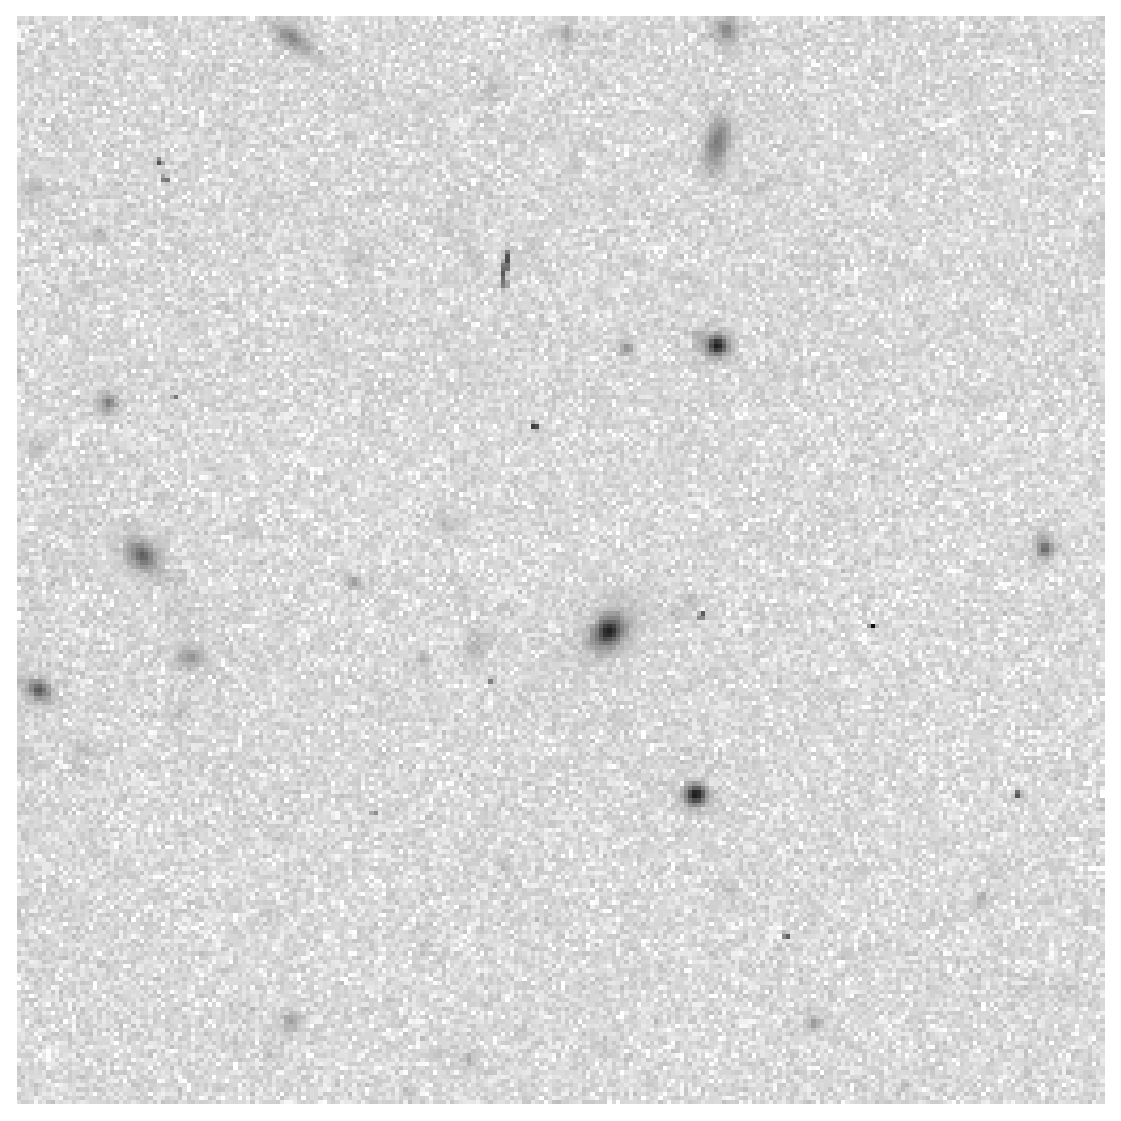
\includegraphics[width=8cm]{ps/cr1.ps}
		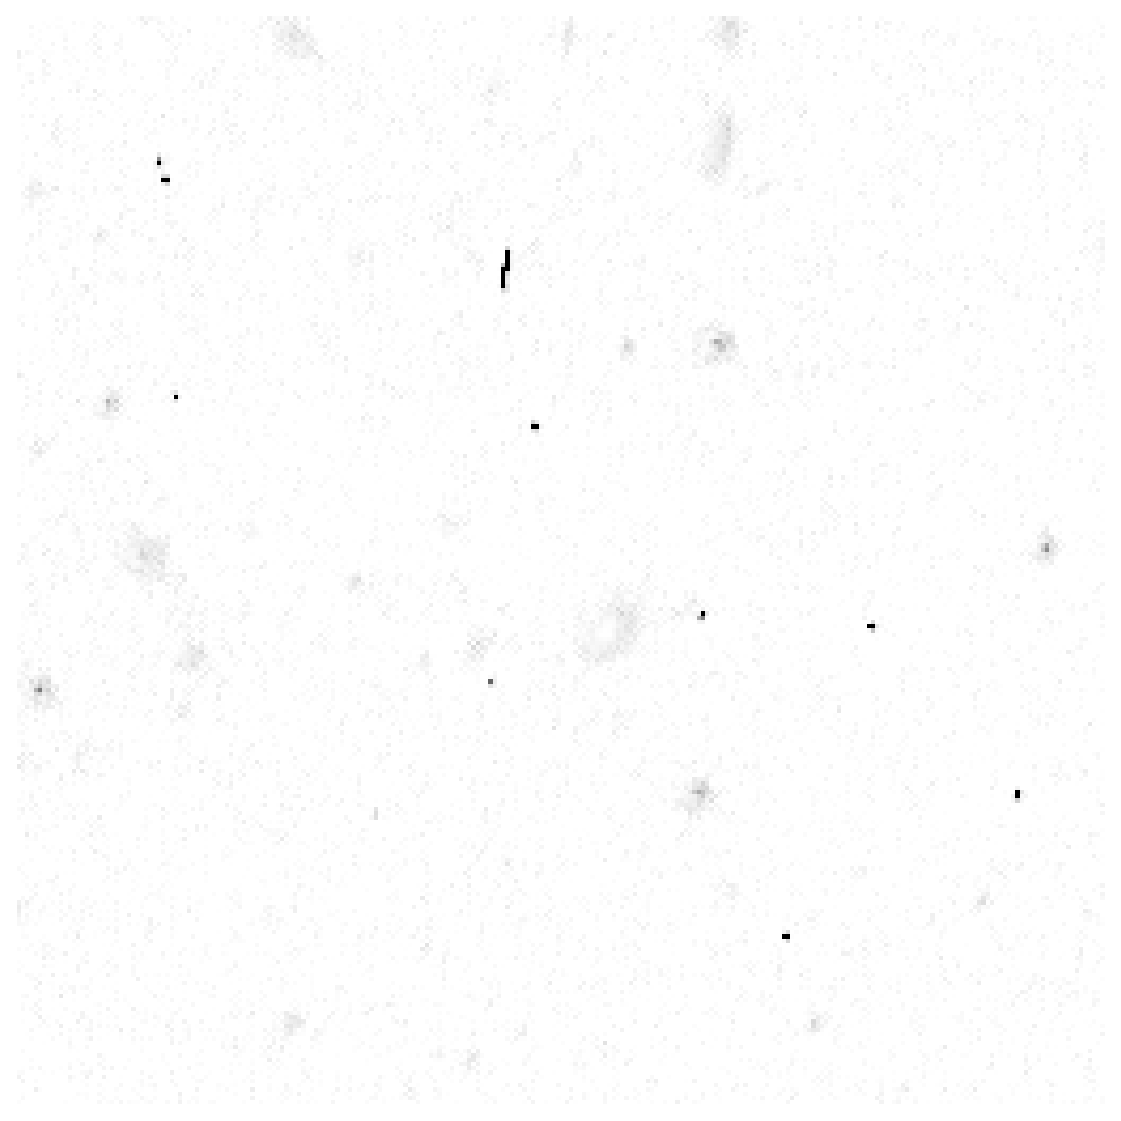
\includegraphics[width=8cm]{ps/cr2.ps}}
      \caption{
              Example of filtering obtained with a retina-filter..
              {\it Left:} Original image (detail). {\it Right:} Filtered
              image (detail).
              }
      \label{fig:result}
   \end{figure}

% \paragraph{Acknowledgments}

\begin{thebibliography}{99}
   \bibitem{bertin} Bertin~E., SExtractor, User's manual, 1999, IAP
   \bibitem{riedmiller:al} Riedmiller~M., Braun~H., 1993, in Proceeding of the
            IEEE Conference on Neural Networks, San Francisco
\end{thebibliography}

\end{document}
